%%%%%%%%%%%%%%%%%%%%%%%%%%%%%%%%%%%%%%%%%
% baposter Portrait Poster
% LaTeX Template
% Version 1.0 (15/5/13)
%
% Created by:
% Brian Amberg (baposter@brian-amberg.de)
%
% This template has been downloaded from:
% http://www.LaTeXTemplates.com
%
% License:
% CC BY-NC-SA 3.0 (http://creativecommons.org/licenses/by-nc-sa/3.0/)
%
%%%%%%%%%%%%%%%%%%%%%%%%%%%%%%%%%%%%%%%%%

%----------------------------------------------------------------------------------------
%	PACKAGES AND OTHER DOCUMENT CONFIGURATIONS
%----------------------------------------------------------------------------------------

\documentclass[a0paper,portrait]{baposter}
\usepackage{cite,url,amsthm,footmisc,bm}
\usepackage{amsmath,graphicx,amssymb,algorithm,algorithmic,graphicx,epsfig,multirow,threeparttable,booktabs,bm,mathdots,tabularx}
\usepackage[font=small,labelfont=bf]{caption} % Required for specifying captions to tables and figures
\usepackage{booktabs} % Horizontal rules in tables
\usepackage{relsize} % Used for making text smaller in some places
\usepackage[percent]{overpic}
\usepackage{natbib}
\usepackage{lipsum}

% The following is for obtaining a rectangle with centered text.
% Remove this if you want the header text to be left justified
% ------------------------------------------
\makeatletter
\renewcommand{\baposter@box@headerdrawtext@rectangle}[1]{
  \path (\baposter@box@name nw) +(0.5\boxwidth,-0.5\baposter@box@@boxheaderheight) node[anchor=center] {#1};%
}
\makeatother
% ------------------------------------------

\graphicspath{{figures/}} % Directory in which figures are stored

\definecolor{bordercol}{RGB}{102,102,255} % Border color of content boxes
\definecolor{headercol1}{RGB}{256,256,256} % Background color for the header in the content boxes (right side) 103 204 247 
\definecolor{headercol2}{RGB}{256,256,256} % Background color for the header in the content boxes (right side)
%\definecolor{headercol2}{RGB}{180,80,80} % Background color for the header in the content boxes (left side)
\definecolor{headerfontcol}{RGB}{0,0,0} % Text color for the header text in the content boxes
\definecolor{boxcolor}{RGB}{256,256,256} % Background color for the content in the content boxes

\begin{document}

\background{ % Set the background to an image (background.pdf)
\begin{tikzpicture}[remember picture,overlay]
\draw (current page.north west)+(-2em,2em) node[anchor=north west]
{
\includegraphics[height=1.1\textheight]{backgroundWhite}};
\end{tikzpicture}
}

\begin{poster}{
grid=false,
borderColor=bordercol, % Border color of content boxes
headerColorOne=headercol2, % Background color for the header in the content boxes (left side)
headerColorTwo=headercol1, % Background color for the header in the content boxes (right side)
headerFontColor=headerfontcol, % Text color for the header text in the content boxes
boxColorOne=boxcolor, % Background color for the content in the content boxes
%headershape=roundedright, % Specify the rounded corner in the content box headers
headerfont=\Large\sf\bf, % Font modifiers for the text in the content box headers
textborder=rectangle,
background=user,
headerborder=open, % Change to closed for a line under the content box headers
boxshade=plain
}
{}
%
%----------------------------------------------------------------------------------------
%	TITLE AND AUTHOR NAME
%----------------------------------------------------------------------------------------
%
{\begin{overpic}[width=\linewidth, grid=false]{header}
 \put (23.5,10) {\Large \textbf{Type Ia Supernovae from non-accreting helium stars}}
 \put (25, 7.5) {\large \textbf{S. Chanlaridis$^{1}$, J. Antoniadis$^{1,2}$, G. Gr\"afener$^{1}$, N. Langer$^{1,2}$}}
 \put (31.5, 5) {\large \textbf{Fundamental Physics in Radio Astronomy}}
 \put (21.5, 3) {\small $^{1}$Argelander-Institut f\"ur Astronomie, Auf dem H\"ugel 71, D-53121 Bonn, Germany}
 \put (19.5, 1) {\small $^{2}$Max-Planck-Institut f\"ur Radioastronomie, Auf dem H\"ugel 69, D-53121 Bonn, Germany}
\end{overpic}}


%----------------------------------------------------------------------------------------
%	INTRODUCTION
%----------------------------------------------------------------------------------------

\headerbox{Abstract}{name=introduction,column=0,row=0, span=3}{
Type Ia supernovae (SNe\,Ia) are luminous optical transients characterized by the absence of hydrogen and helium in their spectra. 
The majority of SNe\,Ia are thought to result from the thermonuclear disruption of white dwarfs, which is triggered by mass accretion in a binary system. 
However, both the details of the explosion mechanism and the exact nature of the progenitor systems remain a topic of debate. 

Recent results from wide-field transient surveys, suggest that SNe\,Ia are far more diverse than previously thought.
This diversity could be the result of varied progenitor systems.
We have discovered a novel SN\,Ia progenitor channel, in which a thermonuclear explosion is initiated during the late evolution of stripped helium stars with masses between $\sim 1.8-2.7$\,M$_{\odot}$ which are frequently produced from the mass donors in interacting massive, close binaries. This mechanism does not require accretion from the binary companion and therefore may contribute significantly to the SN\,Ia rate in star-forming galaxies (i.e. at early delay times). 

}

%----------------------------------------------------------------------------------------
%	MATERIALS AND METHODS
%----------------------------------------------------------------------------------------

\headerbox{Methods \& Initial Parameters}{name=methods,column=0,below=introduction}{
Our numerical stellar models are constructed using the \textbf{M}odules for \textbf{E}xperiments in \textbf{S}tellar \textbf{A}strophysics \citep{Paxton2011}.
\newline
\newline
For the first time, we follow the evolution of low-mass helium stars, from core helium burning to the onset of degenerate oxygen ignition, taking into account important aspects of input physics. More specifically, we employ: 


\begin{itemize}
    \item a reaction network of 43 isotopes, including species that may significantly affect the temperature of the core at high densities,  e.g., those participating in Urca cooling, 
    (${\rm ^{25}Na, ^{25}Mg, ^{23}Na, ^{23}Ne,^{25}Na, ^{25}Ne}$) or,   in exothermic electron-capture reactions (${\rm ^{24}Mg, ^{24}Na, ^{20}Ne, ^{20}F,^{20}O}$),
    
    \item up-to-date weak reaction rates for nuclei with $A = 17-28$, relevant to high-density ONeMg cores \citep{Suzuki2016}
    
    \item an exponentially decreasing diffusive model for convective overshooting \citep{Herwig2000}
    
    \item  stellar wind and convection recipes that allow us  to follow the evolution through a highly unstable super-AGB phase, during which the envelope becomes dynamically unstable, leading to super-Eddington mass-loss rates. 
        
\end{itemize}


We explore a stellar model grid that covers the following parameters: 
%\\[0.5cm]

 \begin{table}[H]
    \caption{Initial model parameters}
    \vspace{-8pt}
    \centering
        \begin{tabular}{cc}
            \hline \hline 
            Parameter & Value(s) \\
            \hline 
            Initial Mass (M$_i$) & $0.8 - 3.5$ M$_{\odot}$\\
            Overshooting ($f_{\text{ov}}$) & $0.0$, $0.014$, $0.016$ \\
            Metallicity ($Z$) & $10^{-4}$, $10^{-3}$, $0.02$ \\
            \hline
        \end{tabular}
\end{table}

}




%----------------------------------------------------------------------------------------
%	RESULTS 1: Residual Carbon
%----------------------------------------------------------------------------------------

\headerbox{Results}{name=results1,span=2,column=1, below=introduction, above=bottom}{ % To reduce this block to 1 column width, remove 'span=2'
Figures\,1 and 2 illustrate a) the core evolution in the $\rho_c - T_c$ plane, and b) the abundance profiles for two representative models before the onset of explosive burning. 

Most models with initial masses between $1.8$ and $2.7$ M$_{\odot}$ develop  degenerate cores composed primarily of oxygen and neon, with a small amount ($\sim 0.01$\,M$_{\odot}$) of residual carbon distributed throughout the core (blue profiles in Figure\,1 and right plot in Figure\,2). 

Subsequent shell burning causes the core to approach the Chandrasekhar limit. When the central density reaches the threshold for electron captures on ${\rm ^{24}Mg}$, the released energy ignites the residual carbon, which in turn leads to explosive core-oxygen burning and, most likely the disruption of the star in a thermonuclear supernova. 


\begin{center}
    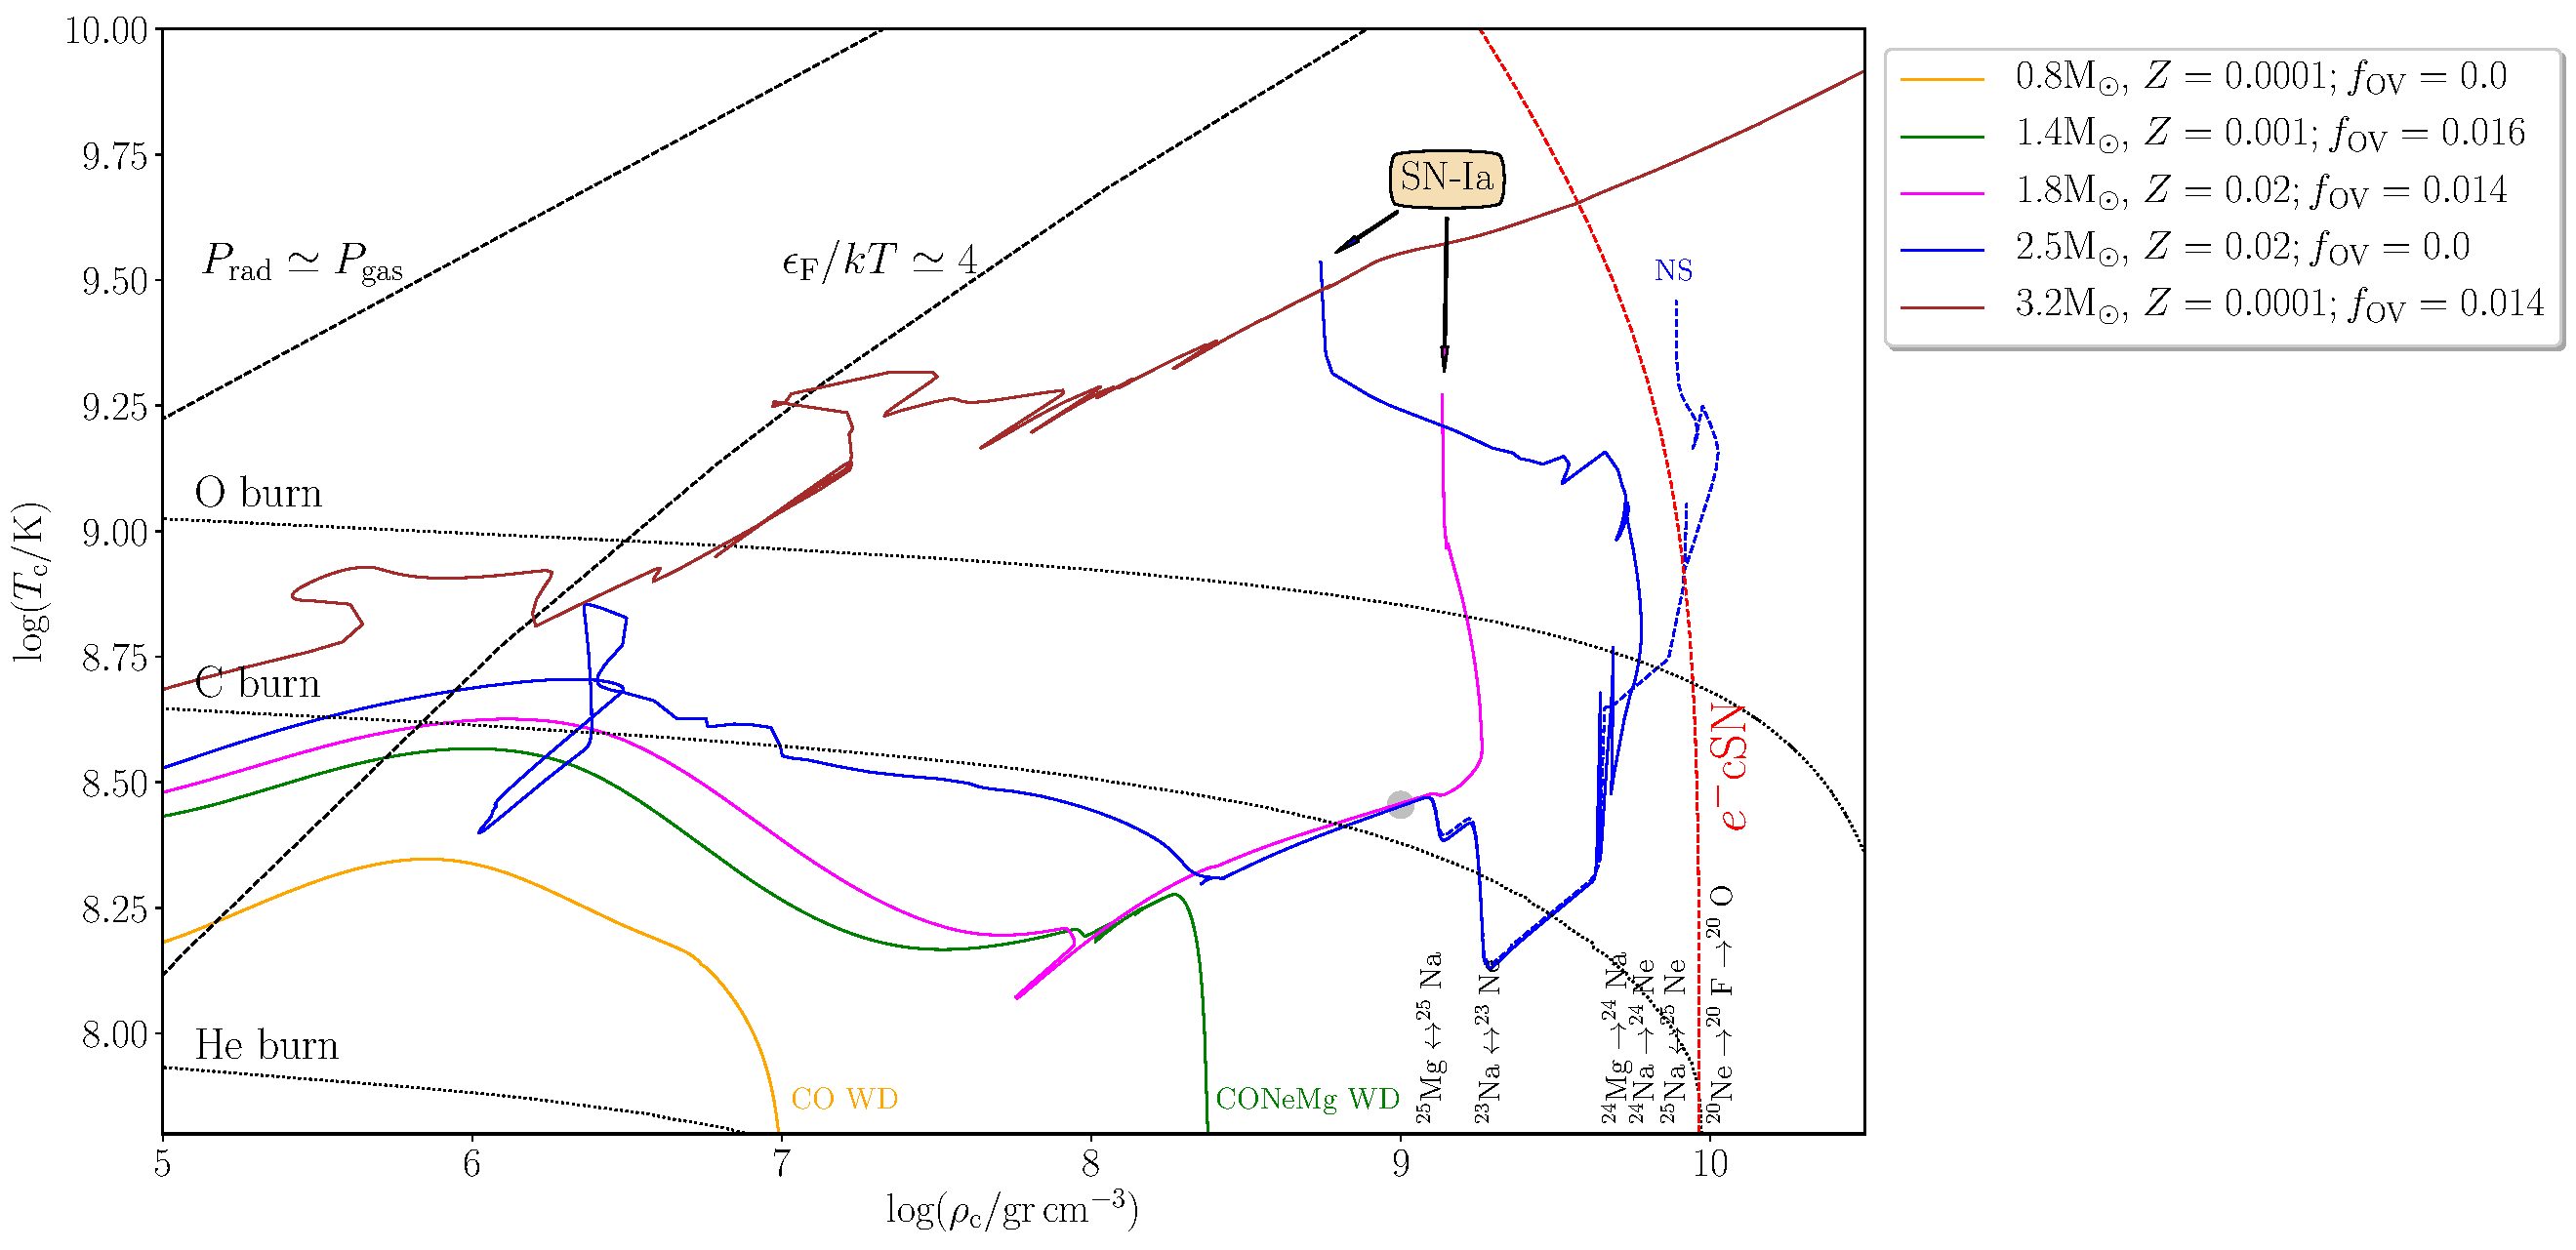
\includegraphics[width=0.85\linewidth]{figures/RhoT.pdf}
    \vspace{-8pt}
    \captionof{figure}{Examples of the evolution of different initial masses in the $\log(\rho_{\rm c})-\log(T_{\rm c})$ plane.  }
\end{center}  
The importance of residual carbon in initiating the explosion is demonstrated by the blue dashed curve in Figure\,1, which shows a model in which all carbon-participating thermonuclear reactions have been switched off. In this case, the core density grows beyond the threshold for e-captures on $^{20}$Ne, most likely leading to an electron-capture supernova and the formation of a neutron star. 



A small number of models develop a hybrid CO/ONe structure in their core, but still reach the Chandrasekhar limit. These models ignite carbon and oxygen explosively at lower densities, and could lead to more energetic explosions (magenta profile in Figure\,1 and left plot in Figure\,2). 
\\[0.57cm]
In all  cases, the extended He-rich stellar envelope is easily ejected, either due a strong wind (as is the case in our single-star models) or, more realistically, in a common-envelope episode with the binary companion.  As a result, the star contains no helium at the time of the explosion, and hence it would be observable as a SN\,Ia (Figure\,2). 




\begin{center}
    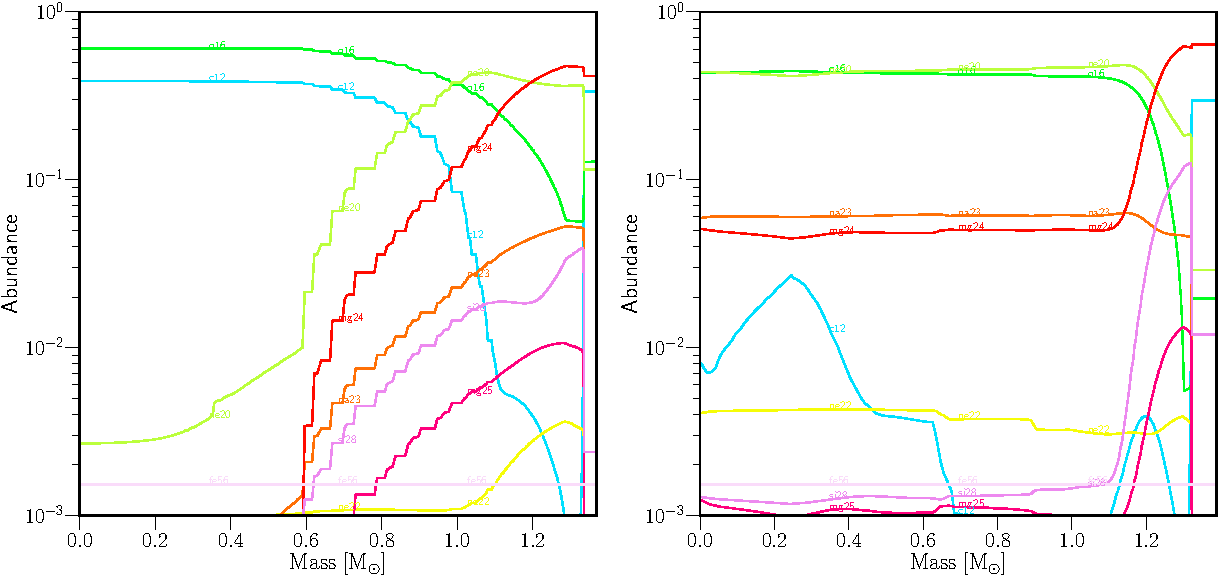
\includegraphics[width=0.85\linewidth]{figures/combineAbun.pdf}
     \captionof{figure}{Structure of two stellar models when $\log(\rho_c) \approx 9.0$, shortly before Urca processes commence (gray circle in Figure\,1). \emph{Left}: Model with initial mass of M$_{i} = 1.8$ M$_{\odot}$, solar metallicity, and overshoot mixing ($\rm f_{OV} = 0.014$). \emph{Right}: Model with M$_{i} = 2.5$ M$_{\odot}$, solar metallicity, and no overshooting. Residual carbon from previous burning stages is visible in the core.}
 \end{center}
}




%----------------------------------------------------------------------------------------
%	REFERENCES
%----------------------------------------------------------------------------------------

\headerbox{References}{name=references,column=0, below=methods, above=bottom}{
\smaller % Reduce the font size in this block
\renewcommand{\section}[2]{\vskip 0.05em} % Get rid of the %default "References" section title
\nocite{*} % Insert publications even if they are not cited in %the poster

\bibliographystyle{unsrt}
\bibliography{sample} % Use sample.bib as the bibliography file
}

\end{poster}

\end{document}